\section{存储访问}

\begin{figure}[H]
    \centering
    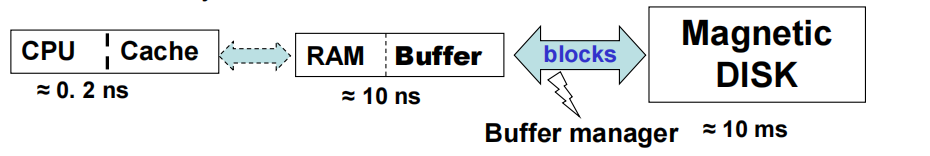
\includegraphics[width=0.8\linewidth]{image6.png}
    \caption{Storage Access}
    \label{}
\end{figure}

\subsection{存储访问}

数据库文件在逻辑上被划分为称为块的固定长度存储单元.块是数据库系统中存储分配和数据传输的单位.

缓冲区:用于存储磁盘块副本的内主存部分.

数据库系统力求最小化磁盘和内存之间的块传输次数.

\begin{itemize}
    \item 为减少磁盘访问次数:在主内存中尽可能多地保留块---缓冲区.
    \item 但缓冲区大小有限,如何处理
\end{itemize}

缓冲区管理区:负责在主内存中分配缓冲区空间的子系统.

\begin{figure}[H]
    \centering
    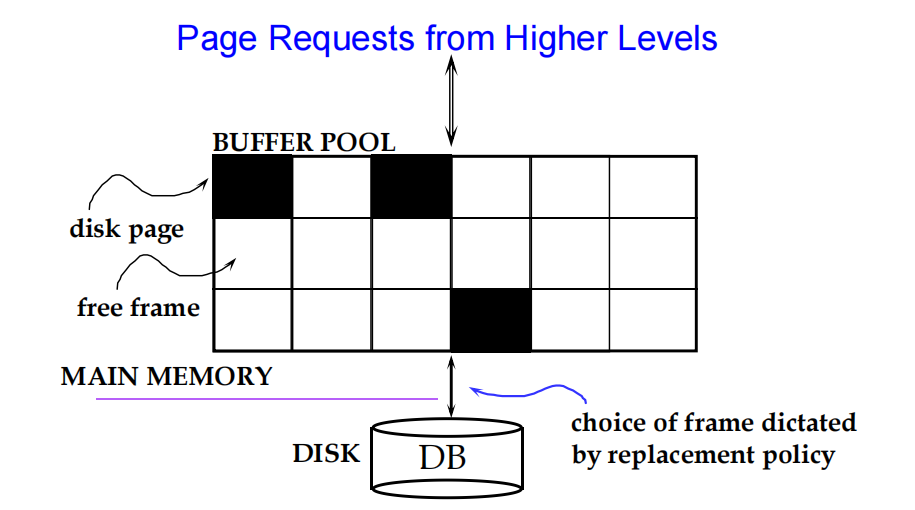
\includegraphics[width=0.8\linewidth]{image7.png}
    \caption{Structure}
    \label{}
\end{figure}

数据必须存于RAM中,DBMS才能对齐进行操作

会维护<frame\#,pageid>对的表格.

页:数据的单位;块:磁盘空间的单位:帧:缓冲池的单位.

\subsection{缓冲区管理器}

应用程序在需要从磁盘获取一个块时会调用Buffer Manager.

\begin{itemize}
    \item 如果该块已在缓冲区中,请求程序将获得该块在主存中的地址
    \item 如果不在缓冲区中:
      \begin{itemize}
         \item 缓冲区管理器在缓冲区中为该块分配空间,替换(丢弃)一些旧页面;如果没有空闲空间,则为新块腾出空间.(在buffer中为新页分配空间).
         \item 只有当被丢弃的块自最近一次写入磁盘或从磁盘读取以来被修改过时,才会将其写回磁盘(将被覆盖的旧块若已被修改过,则写回磁盘).
         \item 一旦在缓冲区中分配了空间,缓冲区管理器就会将数据块从磁盘读取到缓冲区,并将该数据块在主存中的地址传递给请求者(从磁盘读入新块放buffer).
      \end{itemize}
\end{itemize}

缓冲区替换策略:LRU(最近最少使用),MRU(最近最多使用).

固定块:不允许写回磁盘的内存块.(如当前块正在被使用时)

立即丢弃策略:一旦处理完某个块的最后一个元组,就立即释放该块占用的空间.(用后立即丢弃)

强制输出块:块的请求者必须解除对其的固定,并指明页面是否已被修改-----为此使用dirty bit.

pool中的页面可能会被多次请求(被多个事务使用):使用一个引用计数,当且仅当引用计数=0时,页面才是替换候选对象.

\subsection{缓冲区替换策略}

当Buffer的空闲区不够,不能容下新读入的Block时,需要将Buffer中原有Block覆盖(替换).主要策略为:

(1) \textbf{LRU策略}:替换最近最少使用的块.

\begin{itemize}
    \item LRU背后的理念:将过去的块引用模式用作对未来引用的预测器.
    \item 查询具有明确的访问模式,数据库系统可以利用用户查询中的信息来预测未来的引用.
    \item 但对于某些涉及重复扫描数据的访问模式,LRU可能是一种糟糕的策略
\end{itemize}

(2) \textbf{MRU策略}:系统必须固定当前正在处理的块.处理完该块的最后一个元组后,该块被解除固定,并成为最近最常用的块.

\begin{itemize}
    \item 缓冲区管理器可以使用关于请求引用特定关系的概率的统计信息:例如,数据字典经常被访问.启发式方法:将数据字典块保留在主内存缓冲区中.
    \item 缓冲区管理器还支持为恢复目的强制输出快.
    \item 采用查询优化器提供的替换策略提示的混合策略更为可取.
\end{itemize}